\section{Design}
\label{sec:design}

In this section, we present the design of \texttt{ACETA} by firstly describing the ETA pipeline and feature generation of Cisco \texttt{Joy}. Then we explain each of the pipeline components of \texttt{ACETA} in detail. 

\subsection{Reference Design - \texttt{Joy}}
As shown in Figure \ref{figure:joy}, the pipeline processing of \texttt{Joy} starts with having the labelled training data collected in packet capture (.pcap) format. Then, using the feature extractor from \texttt{Joy}, the raw data is processed to generate flow level statistics, which is then used to form the features in a structured JSON format. At this point the user can solicit which features to use on the model for training and classification of samples. Once the data features for each of the samples are prepared, a model is trained, tested, and saved for further inference.

\begin{figure}[h!]
  \centering
  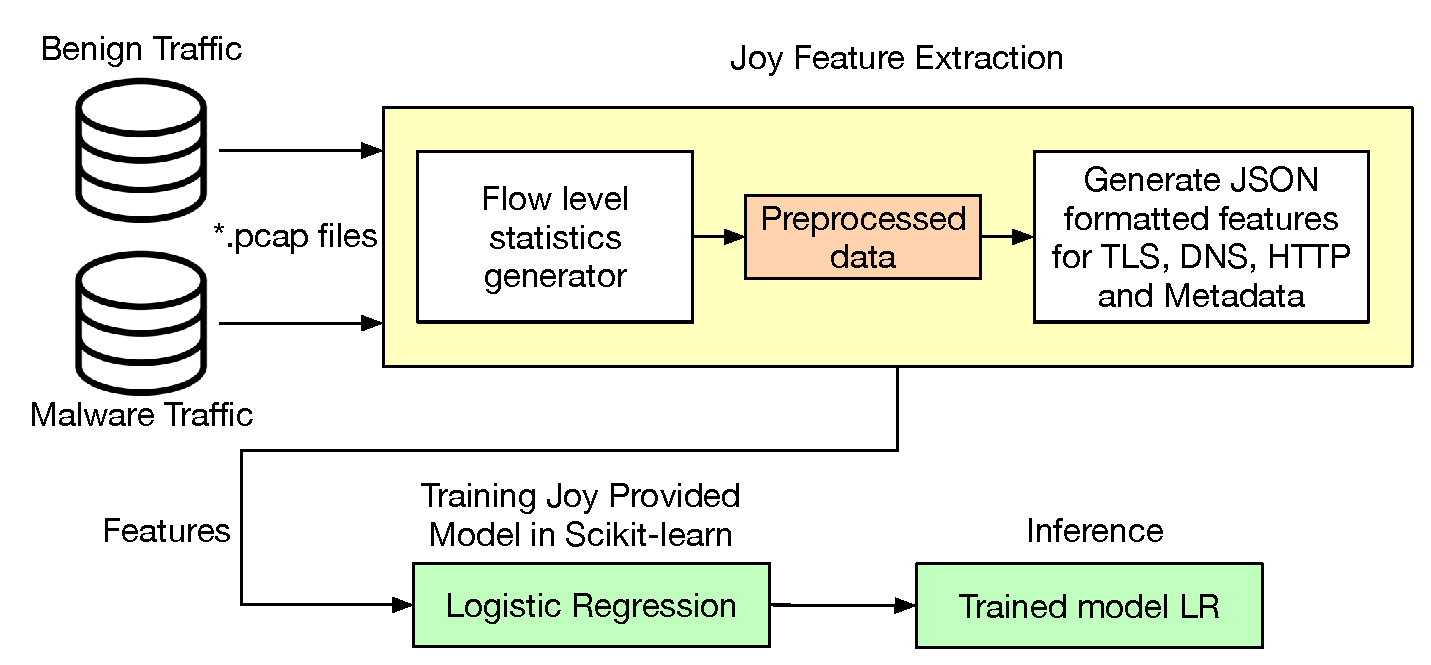
\includegraphics[width=3.3in]{./fig/joy-pipeline.eps}
  \caption{ETA Pipeline of Cisco \texttt{Joy}}
  \label{figure:joy}
\end{figure}

\subsection{Features}

The feature extractor of \texttt{Joy} is capable of extracting TLS, DNS, HTTP and metadata features from network flows. The TLS client-based features are the list of offered ciphersuites, advertised extensions, and the client's public key length, while the server-side TLS features are the selected ciphersuite, supported extensions, number of certificates, number of SAN names, validity in days, and the existence of a self-signed certificate. The DNS flow data is gathered from the corresponding DNS response to the TLS flow. From this flow the gathered features are the lengths of both the domain name and FQDN, the 32 most common TTL values, and binary features representing whether the domain name was in the top-100, top-1,000, top-10,000, top-100,000, top-1,000,000, or not contained in the Alexa list. HTTP data is collected from the source address of every TLS flow. Seven main types of features are used out of the flow data, which are the presence of outbound and inbound HTTP fields, Content-Type, User-Agent, Accept-Language, Server, and code. For metadata, features include the sequence of packet lengths, inter-arrival times, and byte distribution. 

A comprehensive list of features used in \texttt{ACETA} can be found from the list below.

\begin{itemize}
	\item
	The TLS features include:
	1) Client advertised ciphersuites;
	2) Client advertised extensions;
	3) Server supported ciphersuites;
	4) Server supported extensions;
	5) Client public key length;
	6) Number of server certificates;
	7) Number of subject alternative names (SAN) of server;
	8) Validity of server certificates; and
	9) Whether the certificate is self signed.
	\item
	The DNS features include: 
	1) Length;
	2) Suffix;
	3) TTL;
	4) Number of numerical character;
	5) Number of Non-alphanumerical character;
	6) Number of IPs returned per request; and
	7) Alexa rank.
	\item
	The HTTP features include:
	1) Presence of HTTP fields;
	2) Content-type;
	3) User-agent;
	4) Server; and
	5) Return code.
	
	\item
	The metadata features include: 
	1) Inter-Packet Times Markov Matrix;
	2) Inter-Packet Lengths Markov Matrix; and
	3) Byte Distribution.
\end{itemize}

\subsection{\texttt{ACETA} Overview}

As shown in the Figure \ref{figure:aceta}, \texttt{ACETA} improves upon the baseline \texttt{Joy} by accelerating the processing steps at different levels. The initial processing with the \texttt{Joy} tool is accelerated by taking advantage of multicore processors, using multithreading. Likewise, each of the feature processing steps are accelerated by using multiple processes as well. The data processing steps of \texttt{ACETA} use JSON files as the structured storage for our processed data. With the large number of reads and writes our tool needs to complete, the standard JSON library was a substantial bottleneck in the data processing pipeline. Using the C optimized Ultra JSON (ujson) library as a drop in replacement, we gain faster processing with identically structured results. With the data prepared, using the Intel Data Analytics Acceleration Library \cite{daal}, we can accelerate the training and testing of models significantly faster than the standard machine learning libraries.

\begin{figure}[h!]
	\centering
	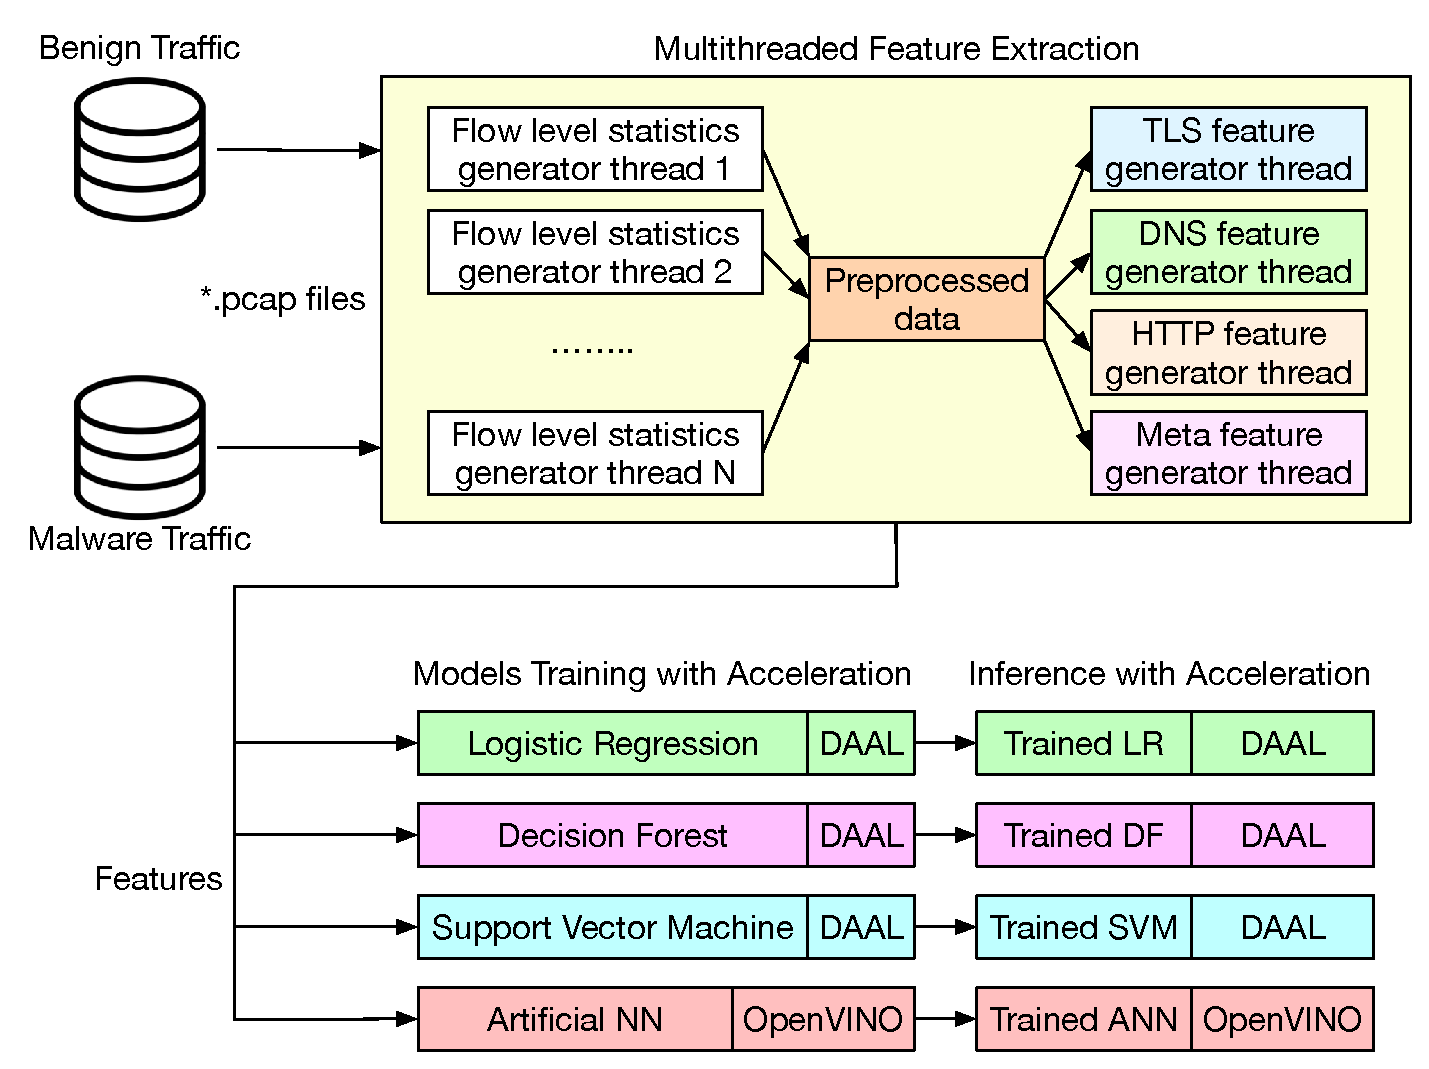
\includegraphics[width=3.3in]{./fig/aceta-pipeline.eps}
	\caption{ETA Pipeline of \texttt{ACETA}}
	\label{figure:aceta}
\end{figure}

\subsection{Acceleration}
Our initial optimizations target the first few data processing steps in \texttt{ACETA}. The performance is enhanced by using several different strategies. First, the code is simplified by implementing faster coding alternatives, such as list comprehensions and conditional exectution using try-catch. Next, the performance libraries Numpy and UltraJSON are implemented for further acceleration. With raw data samples being separated into their unique malware/benign family folders, the organizational structure of the raw data is established effectively to be processed in parallel. Using the multiprocessing library, the parallel capability of multicore machines are leveraged for additional performance gains.

After processing the raw data, the primary focus is on accelerating the model training and inference. The Intel Data Analytics Acceleration Library (DAAL)  \cite{daal} provides optimized machine learning routines and algorithms targeted for Intel processors. DAAL functions maximize processing speed by knowing the instruction set, vector width, core counts, and memory architecture for each processor they run on. Similar to the popular Scikit-learn library, DAAL offers support for many of the popular machine learning algorithms. For our purposes, we compare logistic regression, decision forest, support vector machine, and neural network, by training on identical datasets with both non-DAAL and DAAL version code.

The DAAL machine learning pipeline was designed closely based off of the current popular libraries' structure, such as Scikit-learn. A code comparison of DAAL vs. Scikit-learn is shown in Algorithms \ref{alg:sklearn-lr} and \ref{alg:daal-lr}. Both algorithms implement the same general pipeline of creating a model, training the model, and then predicting using the trained model. This similarity makes implementing DAAL into code that uses one of the standard libraries as simple as possible. 

\begin{algorithm}[h!]
	\caption{Scikit-learn code}
	\scriptsize
	\begin{algorithmic}[1]
		\State import sklearn
		\State logreg = sklearn.linear\_model.LogisticRegression(parameters)
		\State logreg.fit(trainData, trainLabels)
		\State predictions = logreg.predict(testData)
	\end{algorithmic}
	\label{alg:sklearn-lr}
\end{algorithm}

\begin{algorithm}[h!]
	\caption{DAAL code}
	\scriptsize
	\begin{algorithmic}[1]
		\State import daal4py
		\State logreg = daal4py.logistic\_regression\_training(parameters)
		\State trainedModel = logreg.compute(trainData, trainLabels)
		\State predictAlg = daal4py.logistic\_regression\_prediction(parameters)
		\State predictResult = predictAlg.compute(testData, trainedModel.model)
		\State predictions = predictResult.prediction
	\end{algorithmic}
	\label{alg:daal-lr}
\end{algorithm}

For deep learning, Intel also offers a dedicated framework, OpenVINO  \cite{openvino}, that optimizes deep learning models in a similar manner to DAAL. OpenVINO has two components, its Model Optimizer and Inference Engine. The optimization process first requires a pre-trained model from one of its supported deep learning frameworks, in our case TensorFlow. First, the TensorFlow must be frozen into a format the Model Optimizer can analyze. The Model Optimizer converts the TensorFlow model to make an optimized intermediate representation based on the trained network topology, weights, and bias values. The newly optimized model is then used by the Inference Engine to classify new data, at a faster rate and with identical accuracy compared to the original TensorFlow model.

